\chapter{An Intuitive Approach to Groups}
\label{chapter:intuitive_approach_groups}
\thispagestyle{empty}

One of the major topics of this course is \textbf{groups}.  The area of mathematics that is concerned with groups is called \textbf{group theory}. Loosely speaking, group theory is the study of symmetry, and in my opinion is one of the most beautiful areas in all of mathematics. It arises in puzzles, visual arts, music, nature, the physical and life sciences, computer science, cryptography, and of course, throughout mathematics.

Instead of starting with an abstract formal definition, we will begin our study of groups by developing some intuition about what groups actually are.  To get started, we will be exploring the game Spinpossible\texttrademark (which used to be available for iOS and Android devices).  The game is played on a $3\times 3$ board of scrambled tiles numbered 1 to 9, each of which may be right-side-up or up-side-down. The objective of the game is to return the board to the standard configuration where tiles are arranged in numerical order and right-side-up. This is accomplished by a sequence of ``spins", where a spin consists of rotating an $m\times n$ subrectangle by 180$^\circ$. The goal is to minimize the number of spins used.  The following figure depicts a scrambled board on the left and the solved board on the right.  The sequence of arrows is used to denote some sequence of spins that transforms the scrambled board into the solved board.

\begin{center}
\begin{tabular}{c}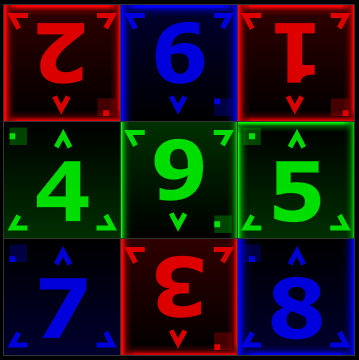
\includegraphics[width=1.5in]{scramble1.PNG}\end{tabular}
{\large $\xrightarrow{?} \cdots \xrightarrow{?}$}
\begin{tabular}{c}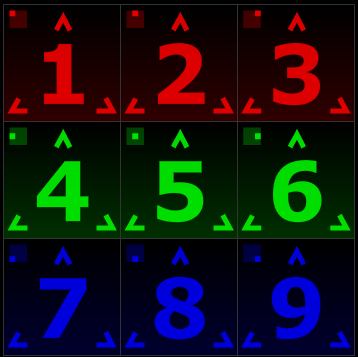
\includegraphics[width=1.5in]{scramble4.PNG}\end{tabular}
\end{center}

\begin{example}\label{ex:spinpossible}
Let's play with an example.  Suppose we start with the following scrambled board.

\begin{center}
\begin{tikzpicture}[every node/.style={minimum size=.65cm}]
  \node [draw] (1) {\rotatebox{180}{$\underline{2}$}};
  \node [draw, right=0cm of 1] (2) {\rotatebox{180}{$\underline{9}$}};
  \node [draw, right=0cm of 2] (3) {\rotatebox{180}{$\underline{1}$}};
  \node [draw, below=0cm of 1] (4) {$\underline{4}$};
  \node [draw, right=0cm of 4] (5) {\rotatebox{180}{$\underline{6}$}};
  \node [draw, right=0cm of 5] (6) {$\underline{5}$};
  \node [draw, below=0cm of 4] (7) {$\underline{7}$};
  \node [draw, right=0cm of 7] (8) {\rotatebox{180}{$\underline{3}$}};
  \node [draw, right=0cm of 8] (9) {$\underline{8}$};
\end{tikzpicture}
\end{center}

\noindent The underlines on the numbers are meant to help us tell whether a tile is right-side-up or up-side-down.  Our goal is to use a sequence of spins to unscramble the board.  Before we get started, let's agree on some conventions.  When we refer to tile $n$, we mean the actual tile that is labeled by the number $n$ regardless of its position and orientation on the board.  On the other hand, position $n$ will refer to the position on the board that tile $n$ is supposed to be in when the board has been unscrambled.  For example, in the board above, tile 1 is in position 3 and tile 7 happens to be in position 7.  

It turns out that there are multiple ways to unscramble this board., but I have one particular sequence in mind.  First, let's spin the rectangle determined by the two rightmost columns.  Here's what we get.  I've shaded the subrectangle that we are spinning.

\begin{center}
\begin{tabular}{c}
\begin{tikzpicture}[every node/.style={minimum size=.65cm}]
  \node [draw] (1) {\rotatebox{180}{$\underline{2}$}};
  \node [draw, fill=blue!40, right=0cm of 1] (2) {\rotatebox{180}{$\underline{9}$}};
  \node [draw, fill=blue!40, right=0cm of 2] (3) {\rotatebox{180}{$\underline{1}$}};
  \node [draw, below=0cm of 1] (4) {$\underline{4}$};
  \node [draw, fill=blue!40, right=0cm of 4] (5) {\rotatebox{180}{$\underline{6}$}};
  \node [draw, fill=blue!40, right=0cm of 5] (6) {$\underline{5}$};
  \node [draw, below=0cm of 4] (7) {$\underline{7}$};
  \node [draw, fill=blue!40, right=0cm of 7] (8) {\rotatebox{180}{$\underline{3}$}};
  \node [draw, fill=blue!40, right=0cm of 8] (9) {$\underline{8}$};
\end{tikzpicture}
\end{tabular}
%
{\large $\rightarrow$}
%
\begin{tabular}{c}
\begin{tikzpicture}[every node/.style={minimum size=.65cm}]
  \node [draw] (1) {\rotatebox{180}{$\underline{2}$}};
  \node [draw, right=0cm of 1] (2) {\rotatebox{180}{$\underline{8}$}};
  \node [draw, right=0cm of 2] (3) {$\underline{3}$};
  \node [draw, below=0cm of 1] (4) {$\underline{4}$};
  \node [draw, right=0cm of 4] (5) {\rotatebox{180}{$\underline{5}$}};
  \node [draw, right=0cm of 5] (6) {$\underline{6}$};
  \node [draw, below=0cm of 4] (7) {$\underline{7}$};
  \node [draw, right=0cm of 7] (8) {$\underline{1}$};
  \node [draw, right=0cm of 8] (9) {$\underline{9}$};
\end{tikzpicture}
\end{tabular}
\end{center}

\noindent Okay, now let's spin the middle column.

\begin{center}
\begin{tabular}{c}
\begin{tikzpicture}[every node/.style={minimum size=.65cm}]
  \node [draw] (1) {\rotatebox{180}{$\underline{2}$}};
  \node [draw, fill=blue!40, right=0cm of 1] (2) {\rotatebox{180}{$\underline{8}$}};
  \node [draw, right=0cm of 2] (3) {$\underline{3}$};
  \node [draw, below=0cm of 1] (4) {$\underline{4}$};
  \node [draw, fill=blue!40, right=0cm of 4] (5) {\rotatebox{180}{$\underline{5}$}};
  \node [draw, right=0cm of 5] (6) {$\underline{6}$};
  \node [draw, below=0cm of 4] (7) {$\underline{7}$};
  \node [draw, fill=blue!40, right=0cm of 7] (8) {$\underline{1}$};
  \node [draw, right=0cm of 8] (9) {$\underline{9}$};
\end{tikzpicture}
\end{tabular}
%
{\large $\rightarrow$}
%
\begin{tabular}{c}
\begin{tikzpicture}[every node/.style={minimum size=.65cm}]
  \node [draw] (1) {\rotatebox{180}{$\underline{2}$}};
  \node [draw, right=0cm of 1] (2) {\rotatebox{180}{$\underline{1}$}};
  \node [draw, right=0cm of 2] (3) {$\underline{3}$};
  \node [draw, below=0cm of 1] (4) {$\underline{4}$};
  \node [draw, right=0cm of 4] (5) {$\underline{5}$};
  \node [draw, right=0cm of 5] (6) {$\underline{6}$};
  \node [draw, below=0cm of 4] (7) {$\underline{7}$};
  \node [draw, right=0cm of 7] (8) {$\underline{8}$};
  \node [draw, right=0cm of 8] (9) {$\underline{9}$};
\end{tikzpicture}
\end{tabular}
\end{center}

\noindent Hopefully, you can see that we are really close to unscrambling the board.  All we need to do is spin the rectangle determined by the tiles in positions 1 and 2.

\begin{center}
\begin{tabular}{c}
\begin{tikzpicture}[every node/.style={minimum size=.65cm}]
  \node [draw, fill=blue!40] (1) {\rotatebox{180}{$\underline{2}$}};
  \node [draw, fill=blue!40, right=0cm of 1] (2) {\rotatebox{180}{$\underline{1}$}};
  \node [draw, right=0cm of 2] (3) {$\underline{3}$};
  \node [draw, below=0cm of 1] (4) {$\underline{4}$};
  \node [draw, right=0cm of 4] (5) {$\underline{5}$};
  \node [draw, right=0cm of 5] (6) {$\underline{6}$};
  \node [draw, below=0cm of 4] (7) {$\underline{7}$};
  \node [draw, right=0cm of 7] (8) {$\underline{8}$};
  \node [draw, right=0cm of 8] (9) {$\underline{9}$};
\end{tikzpicture}
\end{tabular}
%
{\large $\rightarrow$}
%
\begin{tabular}{c}
\begin{tikzpicture}[every node/.style={minimum size=.65cm}]
  \node [draw] (1) {$\underline{1}$};
  \node [draw, right=0cm of 1] (2) {$\underline{2}$};
  \node [draw, right=0cm of 2] (3) {$\underline{3}$};
  \node [draw, below=0cm of 1] (4) {$\underline{4}$};
  \node [draw, right=0cm of 4] (5) {$\underline{5}$};
  \node [draw, right=0cm of 5] (6) {$\underline{6}$};
  \node [draw, below=0cm of 4] (7) {$\underline{7}$};
  \node [draw, right=0cm of 7] (8) {$\underline{8}$};
  \node [draw, right=0cm of 8] (9) {$\underline{9}$};
\end{tikzpicture}
\end{tabular}
\end{center}

\noindent Putting all of our moves together, here is what we have.

\begin{center}
\begin{tabular}{c}
\begin{tikzpicture}[every node/.style={minimum size=.65cm}]
  \node [draw] (1) {\rotatebox{180}{$\underline{2}$}};
  \node [draw, fill=blue!40, right=0cm of 1] (2) {\rotatebox{180}{$\underline{9}$}};
  \node [draw, fill=blue!40, right=0cm of 2] (3) {\rotatebox{180}{$\underline{1}$}};
  \node [draw, below=0cm of 1] (4) {$\underline{4}$};
  \node [draw, fill=blue!40, right=0cm of 4] (5) {\rotatebox{180}{$\underline{6}$}};
  \node [draw, fill=blue!40, right=0cm of 5] (6) {$\underline{5}$};
  \node [draw, below=0cm of 4] (7) {$\underline{7}$};
  \node [draw, fill=blue!40, right=0cm of 7] (8) {\rotatebox{180}{$\underline{3}$}};
  \node [draw, fill=blue!40, right=0cm of 8] (9) {$\underline{8}$};
\end{tikzpicture}
\end{tabular}
%
{\large $\rightarrow$}
%
\begin{tabular}{c}
\begin{tikzpicture}[every node/.style={minimum size=.65cm}]
  \node [draw] (1) {\rotatebox{180}{$\underline{2}$}};
  \node [draw, fill=blue!40, right=0cm of 1] (2) {\rotatebox{180}{$\underline{8}$}};
  \node [draw, right=0cm of 2] (3) {$\underline{3}$};
  \node [draw, below=0cm of 1] (4) {$\underline{4}$};
  \node [draw, fill=blue!40, right=0cm of 4] (5) {\rotatebox{180}{$\underline{5}$}};
  \node [draw, right=0cm of 5] (6) {$\underline{6}$};
  \node [draw, below=0cm of 4] (7) {$\underline{7}$};
  \node [draw, fill=blue!40, right=0cm of 7] (8) {$\underline{1}$};
  \node [draw, right=0cm of 8] (9) {$\underline{9}$};
\end{tikzpicture}
\end{tabular}
%
{\large $\rightarrow$}
%
\begin{tabular}{c}
\begin{tikzpicture}[every node/.style={minimum size=.65cm}]
  \node [draw, fill=blue!40] (1) {\rotatebox{180}{$\underline{2}$}};
  \node [draw, fill=blue!40, right=0cm of 1] (2) {\rotatebox{180}{$\underline{1}$}};
  \node [draw, right=0cm of 2] (3) {$\underline{3}$};
  \node [draw, below=0cm of 1] (4) {$\underline{4}$};
  \node [draw, right=0cm of 4] (5) {$\underline{5}$};
  \node [draw, right=0cm of 5] (6) {$\underline{6}$};
  \node [draw, below=0cm of 4] (7) {$\underline{7}$};
  \node [draw, right=0cm of 7] (8) {$\underline{8}$};
  \node [draw, right=0cm of 8] (9) {$\underline{9}$};
\end{tikzpicture}
\end{tabular}
%
{\large $\rightarrow$}
%
\begin{tabular}{c}
\begin{tikzpicture}[every node/.style={minimum size=.65cm}]
  \node [draw] (1) {$\underline{1}$};
  \node [draw, right=0cm of 1] (2) {$\underline{2}$};
  \node [draw, right=0cm of 2] (3) {$\underline{3}$};
  \node [draw, below=0cm of 1] (4) {$\underline{4}$};
  \node [draw, right=0cm of 4] (5) {$\underline{5}$};
  \node [draw, right=0cm of 5] (6) {$\underline{6}$};
  \node [draw, below=0cm of 4] (7) {$\underline{7}$};
  \node [draw, right=0cm of 7] (8) {$\underline{8}$};
  \node [draw, right=0cm of 8] (9) {$\underline{9}$};
\end{tikzpicture}
\end{tabular}
\end{center}
In this case, we were able to solve the scrambled board in 3 moves.  It's not immediately obvious, but it turns out that there is no way to unscramble the board in fewer than 3 spins.  However, there is at least one other solution that involves exactly 3 spins.  We won't worry about proving this; right now we are just trying to gain some intuition.

\end{example}

\begin{exercise}
Without worrying about whether your solution is optimal, try to find a different sequence of spins that unscrambles the initial board in Example~\ref{ex:spinpossible}.  Your answer should be a sequence of spins.  Describe your sequence in a way that makes sense. Can you find a sequence of 3 spins that is different from the one described in Example~\ref{ex:spinpossible} that unscrambles the board?
\end{exercise}

\begin{exercise}\label{exer:number_spinpossible_boards}
How many scrambled $3\times 3$ Spinpossible boards are there?  To answer this question, you will need to rely on some counting principles such as factorials. \emph{Note:} In this context, we want to include the solved board as one of the scrambled boards. It's just not very scrambled.
\end{exercise}

\begin{exercise}
A natural question to ask is whether every possible scrambling of a board in Spinpossible can be unscrambled using only spins.  It turns out that the answer is yes.  Justify this fact by describing an algorithm that will always unscramble a scrambled board.  It does not matter whether your algorithm is efficient.  That is, we don't care how many steps it takes to unscramble the board as long as it works in a finite number of steps.  Also, if it didn't occur to you yet, we can always spin a single tile (referred to as \emph{toggling} a tile).
\end{exercise}

\begin{exercise}
Does the order in which you apply spins matter?  Does it always matter?  Let's be as specific as possible.  If the order in which we apply two spins does not matter, then we say that the spins \textbf{commute}.  However, if the order does matter, then the spins do not commute.  When will two spins commute?  When will they not commute?  Provide some specific examples.
\end{exercise}

\begin{exercise}\label{exer:counting_spins}
How many possible spins are there?  We are referring to the moves you are allowed to do at any stage in the game.  Don't forget that you are allowed to toggle a single tile.
\end{exercise}

In a 2011 paper, Alex Sutherland and Andrew Sutherland (a father and son team) present a number of interesting results about Spinpossible and list a few open problems. You can find the paper at \url{http://arxiv.org/abs/1110.6645}. As a side note, Alex is one of the developers of the game and his father, Andrew, is a mathematics professor at MIT. Using a brute-force computer algorithm, the Sutherlands verified that every scrambled $3\times 3$ board can be solved in at most 9 moves. However, a human readable mathematical proof of this fact remains elusive.  By the way, mathematics is chock full of open problems and you can often get to the frontier of what is currently known without too much trouble.  Mathematicians are in the business of solving open problems.

At least for now, let's ignore the optimality requirement of the game.  That is, let's not worry about how many spins it takes to solve a scrambled board.  It turns out that we can ``build" some spins from other spins.  As an example, if I wanted to toggle the tile in position 2, I could first spin the rectangle determined by positions 1 and 2, then toggle the tile in position 1, and lastly spin the rectangle determined by positions 1 and 2 again.  Of course, this is horribly inefficient, but it works.  Also, it is important to point out that I was describing the tile positions we were spinning while not paying any attention to the tiles occupying the corresponding positions.

It's not too difficult to prove that we can build all of the possible spins by only using the following spins.  I've listed some shorter names for these spins in parentheses.
\begin{enumerate}
\item Toggle position 1 ($t$),
\item Spin rectangle determined by positions 1 and 2 ($s_1$),
\item Spin rectangle determined by positions 2 and 3 ($s_2$),
\item Spin rectangle determined by positions 3 and 6 ($s_3$),
\item Spin rectangle determined by positions 6 and 5 ($s_4$),
\item Spin rectangle determined by positions 5 and 4 ($s_5$),
\item Spin rectangle determined by positions 4 and 7 ($s_6$),
\item Spin rectangle determined by positions 7 and 8 ($s_7$),
\item Spin rectangle determined by positions 8 and 9 ($s_8$).
\end{enumerate}
We can describe any of the allowable spins in the game by writing down a sequence consisting of $t,s_1, s_2,\ldots, s_8$.

\begin{example}
Spinning the subrectangle determined by positions 1 and 4 is an allowable spin, but it's not on our list above. We can build this spin by using the following sequence of spins: 
\[
s_1\to s_2\to s_3\to s_4\to s_5\to s_4\to s_3\to s_2\to s_1.
\]
\end{example}

\begin{exercise}
Toggling the tile in position 3 is an allowable spin. Try to find a sequence of spins involving $t, s_1, s_2, \ldots, s_8$ only that yields this toggle.
\end{exercise}

In addition to building all of the allowable spins, we can also describe any possible rearrangement of tiles (position and/or orientation) using just these 9 spins.  For example, if we apply $s_2$, followed by $s_3$, and then $s_2$ again, the net result is swapping the tiles in positions 2 and 6 while maintaining their orientation.  You should take the time to verify this. However, notice that the net action is \emph{not} an allowable spin.  That is, not every sequence of the 9 spins $t, s_1, s_2,\ldots, s_8$ results in an allowable spin.  

\begin{exercise}
What is the net action of applying $s_1$, then $s_2$, and then $s_1$?  Is the net action an allowable spin?  How about $s_2$, then $s_1$, and then $s_2$?
\end{exercise}

We say that the set $\{t, s_1,\ldots,s_8\}$ \textbf{generates} all possible scramblings of the $3\times 3$ board. In this case, we refer to $\{t, s_1,\ldots,s_8\}$ as a set of \textbf{generators}. It turns out that this generating set is minimal in the sense that if we tried to get rid of any one of $t, s_1, \ldots, s_8$, we would no longer be able to generate all scramblings.  Note that there are other minimal generating sets and there are lots of sets that will generate all the scramblings that are not minimal.

We need to establish some conventions about how to write down sequences of spins involving the generators.  Since we are doing spins on top of spins, we will follow the convention of function notation that says the function on the right goes first.  For example, $ts_1 s_3$ means do $s_3$ first, then do $s_1$, and lastly do $t$.  This will take some getting used to, but just remember that it is just like function notation (stuff on the right goes first).  We will refer to sequences like $ts_1 s_3$ as \textbf{words} in the generators $t,s_1,\ldots, s_8$. We can also use exponents to abbreviate.  For example, $s_2^2$ is the same as $s_2 s_2$ (which in this case has the net action of doing nothing) and $(s_1 s_2)^2$ is the same as $s_1 s_2 s_1 s_2$.

\begin{exercise}
It turns out that there is an even simpler word (i.e., a shorter word) that yields the same net action as $(s_1 s_2)^2$. Can you find one?
\end{exercise}

\begin{exercise}
Try to write the spin that rotates the entire top row (i.e., spin the top row) as a sequence of moves involving only $t, s_1, \ldots, s_8$.
\end{exercise}

Let's make a couple more observations.  First, every spin is reversible (i.e., has an \emph{inverse}).  In this case, we could just apply the same spin again to undo it.  For example, $s_1^2$ is the same as doing nothing. This means that the reverse of $s_1$, denoted $s_1^{-1}$, is $s_1$ itself. Symbolically, we write $s_1^{-1}=s_1$.  \emph{Warning:} Remember that we are exploring the game Spinpossible; it won't always be the case that repeating a generator will reverse the action. In the same vein, every sequence of spins is reversible. For example, if we apply $s_1 s_2$ (remember that's do $s_2$ first and then $s_1$) to some scrambled board, we could undo the net action by applying $s_2 s_1$.  That is, the reverse (or inverse) of $s_1 s_2$ is $s_2 s_1$. Written symbolically, we have
\[
(s_1 s_2)^{-1}=s_2^{-1} s_1^{-1}=s_2 s_1
\]
since $s_2^{-1}=s_2$ and $s_1^{-1}=s_1$.

\begin{exercise}
Imagine we started with a scrambled board and you were then able to unscramble the board using some sequence from $t, s_1, \ldots, s_8$.  In this case, you would have some word in $t, s_1, \ldots, s_8$ (with repeats allowed). Let's call it $w$.  Now, imagine you have the solved board.  How could you obtain the scrambled board that $w$ unscrambled using only $t, s_1,\ldots, s_8$? How is this related to $w^{-1}$?
\end{exercise}

The upshot of the previous exercise is that the action of any sequence of generators can be reversed and is itself an action.

At this time, I think we are ready to summarize some of our observations of the game Spinpossible and to make a few general claims, which we will state as a list of rules.

\begin{description}
\item[Rule 1.] There is a predefined list of actions that never changes.
\item[Rule 2.] Every action is reversible.\footnote{Implicit in this rule is that the reverse of an action is also an action.}
\item[Rule 3.] Every action is deterministic.
\item[Rule 4.] Any sequence of consecutive actions is also an action.
\end{description}

Rule 1 states that we must start with some fixed set of actions. These are our generators.  In the case of Spinpossible, we encountered two possible generating sets.  First, there was the set of allowable spins, which you counted in Exercise~\ref{exer:counting_spins}.  Second, we considered the set $\{t,s_1,\ldots, s_8\}$, which is a much smaller list of predefined actions.

Rule 2 tells us that every action given in Rule 1 has an inverse. In the case of Spinpossible, every predefined spin is its own inverse.

By deterministic, we mean that we know exactly what will happen when we apply an action.  In contrast, pulling a card off the top of a shuffled deck of cards is not deterministic because we don't know which card we will end up with. Certainly, every spin is deterministic. For example, if we apply $s_6$, we know exactly what will happen.

Rule 4 provides us with a way to build new actions from the actions given in Rule 1.  For example, if we are given $\{t,s_1,\ldots, s_8\}$ as our predefined list of actions (Rule 1), then Rule 4 guarantees that $s_1 s_2 s_3 t$ is also an action (but does not have to be a spin).

\begin{exercise}
Notice that there is no explicit rule that says that every sequence of consecutive actions is reversible.  Is this a consequence of Rules 1--4?  Explain your answer.
\end{exercise}

Alright, we are finally ready for our intuitive and unofficial definition of a group.

\begin{intuitivedef}\label{def:informal_group}
A \textbf{group} is a system or collection of actions that satisfies Rules 1--4 above.
\end{intuitivedef}

Our first example of a group is the set of actions that rearranges and reorients the tiles on the $3\times 3$ Spinpossible board.  Notice that I didn't say that the set of scrambled boards was a group.  It turns out that there is a one-to-one correspondence between actions for Spinpossible and scrambled boards, but for now let's focus on the actions.

\begin{exercise}
Describe how the Rubik's Cube fits into the framework of Rules 1--4.
\end{exercise}

\begin{exercise}\label{exer:2coins}%Modification of Exercise 1.1 in 1.5 of VGT
Place two coins side by side on a table.  Consider just one predefined action: swapping the positions of the two coins.  Can we form a group of actions using this one action as our starting point?  If so, completely describe the collection of actions.  If not, explain why.
\end{exercise}

\begin{exercise}%Modification of Exercise 1.2 in 1.5 of VGT
Consider Exercise~\ref{exer:2coins}, but add a third coin to the right of the other two coins.  The only predefined action is still the one from the previous exercise: swapping the positions of the two leftmost coins.  Can we form a group of actions using this one action as our starting point?  If so, completely describe the collection of actions. If not, explain why.  How does your answer to this exercise compare to the previous?
\end{exercise}

\begin{exercise}
Consider your three coins from the previous exercise.  Now, for your actions take all possible actions of rearranging the coins.  It turns out that this is a group.
\begin{enumerate}[label=\rm{(\alph*)}]
\item\label{do-nothing} One of the actions is to swap the second and third coins.  What happens if you do this action twice?  Is this an action?  
\item How many actions does this group have?  Describe them all.
\item Can you think of a small set of actions that would generate all the other actions?  Can you find a minimal one (in the sense that removing one of your initial actions would result in a different group)?  Write each of the actions of this group as a word in your generators?  Do some actions have more than one word representing it?
\end{enumerate}
\end{exercise}

In part \ref{do-nothing} of the previous exercise you encountered the ``do-nothing" action, which we will refer to as the \textbf{identity} of the group.

\begin{exercise}
Explain why every group has a do-nothing action (i.e., an identity).
\end{exercise}

\begin{exercise}%Exercise 1.3 in in 1.5 of VGT
Imagine you have 10 coins in your left pocket.  Consider two actions: (1) move a coin from your left pocket to your right pocket, and (2) move a coin from your right pocket to your left pocket.  Is this a group?  Explain your answer.
\end{exercise}

\begin{exercise}
Imagine you have a square puzzle piece that fits perfectly in a square hole.  Consider these actions: pick up the square and rotate it an appropriate amount so that it fits back in the hole.  Is this a group?  Explain your answer.  If it is a group, how many distinct actions are there?
\end{exercise}

\begin{exercise}
Can you describe a group that has exactly $n$ actions for any natural number $n$?
\end{exercise}

\begin{exercise}
Can you describe a situation that satisfies Rules 1--3, but not Rule 4?
\end{exercise}

\begin{exercise}\label{exer:introducing_Z}%Exercise 1.14 in in 1.5 of VGT
Pick your favorite integer.  Consider these actions: add any integer to the one you chose.  This is an infinite set of actions.  Is this a group?  If so, how small a set of generators can you find?
\end{exercise}

\begin{exercise}
Consider the previous exercise, but this time multiply instead of add.  Is this a group?  Explain your answer.
\end{exercise}